
\chapter{Diseño e implementación} % Main chapter title
En este capitulo se abordara la descripcion de la arquitectura general del sistema, arquitectura del firmware, detalles de los controladores desarrollados para el modulo de comunicaicon y los sensores, desarrollo del hardware y la configuracion de la plataforma IoT. 
\label{Chapter3} % Change X to a consecutive number; for referencing this chapter elsewhere, use \ref{ChapterX}

\definecolor{mygreen}{rgb}{0,0.6,0}
\definecolor{mygray}{rgb}{0.5,0.5,0.5}
\definecolor{mymauve}{rgb}{0.58,0,0.82}

%%%%%%%%%%%%%%%%%%%%%%%%%%%%%%%%%%%%%%%%%%%%%%%%%%%%%%%%%%%%%%%%%%%%%%%%%%%%%
% parámetros para configurar el formato del código en los entornos lstlisting
%%%%%%%%%%%%%%%%%%%%%%%%%%%%%%%%%%%%%%%%%%%%%%%%%%%%%%%%%%%%%%%%%%%%%%%%%%%%%
\lstset{ %
  backgroundcolor=\color{white},   % choose the background color; you must add \usepackage{color} or \usepackage{xcolor}
  basicstyle=\footnotesize,        % the size of the fonts that are used for the code
  breakatwhitespace=false,         % sets if automatic breaks should only happen at whitespace
  breaklines=true,                 % sets automatic line breaking
  captionpos=b,                    % sets the caption-position to bottom
  commentstyle=\color{mygreen},    % comment style
  deletekeywords={...},            % if you want to delete keywords from the given language
  %escapeinside={\%*}{*)},          % if you want to add LaTeX within your code
  %extendedchars=true,              % lets you use non-ASCII characters; for 8-bits encodings only, does not work with UTF-8
  %frame=single,	                % adds a frame around the code
  keepspaces=true,                 % keeps spaces in text, useful for keeping indentation of code (possibly needs columns=flexible)
  keywordstyle=\color{blue},       % keyword style
  language=[ANSI]C,                % the language of the code
  %otherkeywords={*,...},           % if you want to add more keywords to the set
  numbers=left,                    % where to put the line-numbers; possible values are (none, left, right)
  numbersep=5pt,                   % how far the line-numbers are from the code
  numberstyle=\tiny\color{mygray}, % the style that is used for the line-numbers
  rulecolor=\color{black},         % if not set, the frame-color may be changed on line-breaks within not-black text (e.g. comments (green here))
  showspaces=false,                % show spaces everywhere adding particular underscores; it overrides 'showstringspaces'
  showstringspaces=false,          % underline spaces within strings only
  showtabs=false,                  % show tabs within strings adding particular underscores
  stepnumber=1,                    % the step between two line-numbers. If it's 1, each line will be numbered
  stringstyle=\color{mymauve},     % string literal style
  tabsize=2,	                   % sets default tabsize to 2 spaces
  title=\lstname,                  % show the filename of files included with \lstinputlisting; also try caption instead of title
  morecomment=[s]{/*}{*/}
}


%----------------------------------------------------------------------------------------
%	SECTION 1
%----------------------------------------------------------------------------------------
\section{Diagrama de bloques general del sistema}

En la figura \ref{fig:Diagrama general del sistema IoT} se muestra el diagrama en bloques general del sistema implementado donde se describe la arquitectura IoT la cual consta de tres capas: percepción, red y aplicación.

\begin{figure}[htbp]
	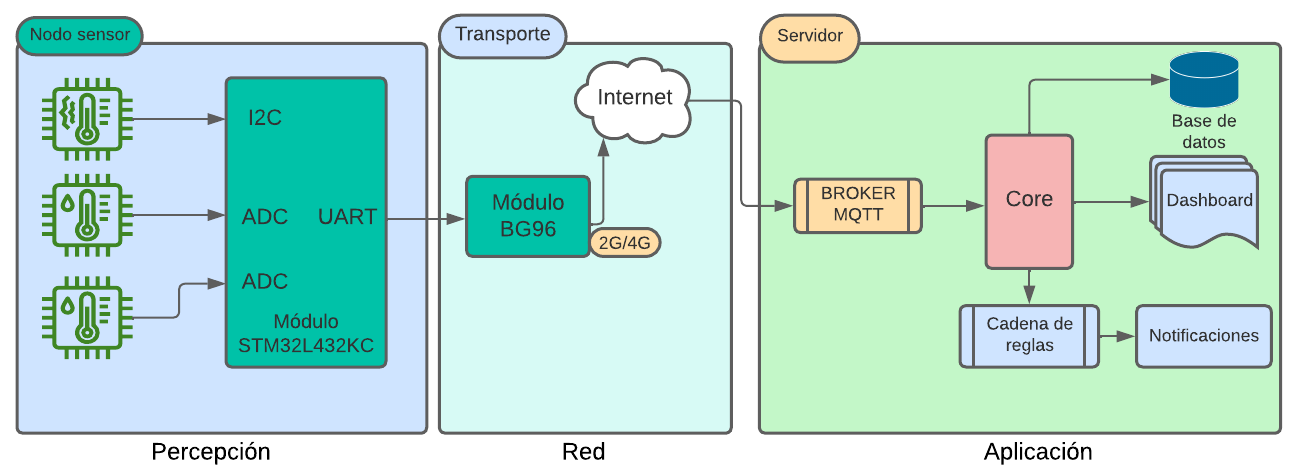
\includegraphics[width=\textwidth, height=8cm]{./Figures/DiagramaDelSistema.png}
	\caption{Diagrama general del sistema IoT.}
	\label{fig:Diagrama general del sistema IoT}
\end{figure}

En cada una de las capas, se despliegan tecnologias y componentes de hardware y software. A continuación se describe cada una de ellas.

\begin{itemize}
	\item Capa de percepción. En la capa de percepción, los nodos sensores son los encargados de medir variables ambientales, hacer un prepocesamiento y enviarlas a la capa de red. Para su desarrollo se utilizo la placa STM32L432KC que contiene el firmware del sistema,tambien consta de un sensor de humedad y temperatrua ambiente AHT10 que se comunica con la placa de desarrollo mediante el protocolo I2C, sensor de humedad de suelo HL-69 y el sensor de luz UV ML-18 que se comunicacion con el modulo mediante entradas analogicas.
  \item Capa de red. En cuanto a la red, se utilizo un modulo quectel BG96 que puede conectarse a la red 2G, 4G, NB-IoT automaticamente dependiendo del nivel de la red en el lugar de la implementacion del modulo sensor, se comunica con el microcontrolador por comandos AT por puerto UART.
  \item Capa de aplicación. En la capa de aplicacion, se utilizo ThingsBoard como plataforma IoT que nos brinda los microservicios de broker MQTT como puerta de entrada al servidor, base de datos para el almacenamiento, nos brinda la interfaz grafica para la visualizacion de los datos y nos permite gestionar la alarmas del sistema.


\end{itemize}

\section{Arquitectura de firmware}
El desarrollo del firmware fue la tarea mas compleja del proyecto debido a que uno de los objetivos fue lograr 
El firmware fue estructurado en capas como se muestra en la figura \ref{fig:Capas del firmware} se dividio el firmware en capas para facilitar el desarrollo y reducir la complejidad del codigo escritolo separo en capas 

\begin{figure}[htbp]
  \centering
	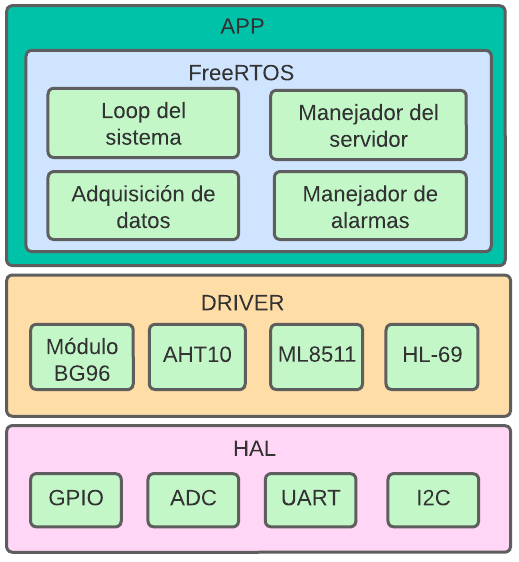
\includegraphics[width=0.7\textwidth]{./Figures/Capas del firmware.png}
	\caption{Capas del firmware.}
	\label{fig:Capas del firmware}
\end{figure}

 La capa Base es la mas baja del sistema y esta compuesta por la libreria HAL de STM, proporciona a las capas superiores la capacidad de interactuar con los perifericos del  microcontrolador STM32L432KC atraves de funciones en lenguaje C
  \begin{itemize}
    \item GPIO: La API proporciona funciones para definir el estado de los pines del microcontrolador.Fueron utilizadas por la capa de APP para el control de los leds de debug del sistema y para el encendido y reset del modulo de comunicacion. Las funciones de esta libreria fue utilizada por la capa de APP para gestionar las entradas y salidas del microcontrolador.
    \item ADC: Proporcionan funciones para la configuracion, lectura y escritura de los pines de microcontroladora senales analogicas. Se utilizaron estas funciones para hacer la lectura de los sensores de humedad de suelo y el sensor de luz UV.
    \item UART: Brinda funciones para la lectura y estritura por el puerto UART del microcontrolador.El firmware utiliza estas funciones para la comunicacion con el modulo BG96.
    \item I2C:Proporciona funciones para la lectura y escritura por protocolo I2C.El driver del sensor de AHT10 utiliza estas funciones para hacer la lectura de los datos.Se utilizaron estas funciones para la lectura de los datos del sensor de AHT10.
    
  \end{itemize}


La capa DRIVERS esta compuesta por los modulos que se desarrollaron para hardware externo al microcontrolador que permiten al microcontrolador enteractuar con hardware externo.Se desarrollaron drivers para el modulo de comunicacion BG96,AHT10,ML18 y HL69
\begin{itemize}
  \item Modulo BG96:Se desarrollo el driver para el modulo BG96, para establecer la comunicacion de este elemento con el microcontrolador a traves del puerto UART.Las funciones mas importantes que proporcionan son
  \begin{itemize}
    \item Estado del modulo.
    \item Descripcion del modulo.
    \item Configuracion APN de la red.
    \item Conexion TCP.
    \item Conexion a broker MQTT.
  \end{itemize}
  \item AHT10: Se desarrollo utilizando la hoja de datos del sensor, proporciona las funciones mas importante inicializacion y lectura de los valores obtenidos por el sensor.
  \item ML18: Se escribio una funcion que permite convertir los datos obtenidos de forma analogica a valores significativos de humedad.
  
\end{itemize}

La capa de APP es la de mayor nivel gerarquico.Se la desarrollo sobre freeRTOS que nos permite hacer un codigo mas escalable.
Se implementaron cuatro tareas
\begin{itemize}
    \item Loop del sistema: Esta tarea es la que nos da la secuencialidad del sistema.
    \item Conexion servidor: Se encarga de manejar la conexion a la red y al broker MQTT.
    \item Adquisicion de datos: Se encarga de hacer la lectura de los sensores.
    \item Manejador de eventos: Esta tarea se encarga de manejar todos lo eventos del sistema.
  \end{itemize}

\section{Desarrollo del firmware}
Para el desarrollo del firmware se utilizo el IDE oficial de STMicroelectronic(STM32CubeIDE).

El firmware fue desarrollado sobre freeRTOS, se utilizaron algunas de sus funcionanlidades como queue, semaforos, tareas, interrupciones.

El firmware tiene una etapa de inicializacion en la figura \ref{fig:Df inicio firmware} podemos ver la secuancia de inicializacion del sistema.

Luego el firmware da el control del sistema al sistema operativo y permanece ejecutando de forma continua las tareas creadas en la etapa de inicializacion del sistema 


En la figura \ref{fig:Df inicio firmware}  se muestra en diagrama de flujo de inicion del firmware.

\begin{figure}[htbp]
  \centering
	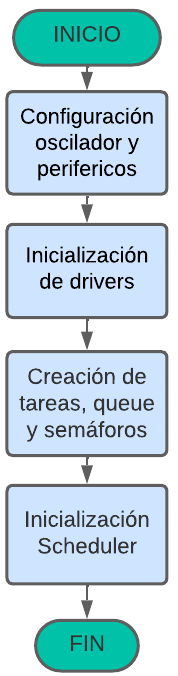
\includegraphics[width=0.25\textwidth]{./Figures/DF inicio firmware.png}
	\caption{Diagrama de flujo inicio firmware.}
	\label{fig:Df inicio firmware}
\end{figure}

Descripcion de los bloques del diagrama.

Lo primero que el firmware realiza es la configuracion del hardware del microcontrolador, luego se inicializan los drivers del modulo de comunicacion celular BG96 y el driver del sensor de humedad AHT10, ejecutan las funciones de inicializacion de los sensores y del modulo de comunicacion celular,posteriormente se crean las tareas, queues y los semaforos del sistema y finalmente se da el contro del sistema al scheduler del sistema operativo. 

Para el control del sistema se crearon cuatro tareas sobre freeRTOS, que se comunican y sincronizan atraves de colas y semaforos en la figura la comunicacion entre tareas.

A continuacion se desarrollara a implementacion de cada tarea del sistema.


La secuencialidad del sistema es manejado por la tarea de loop que nos permite tener secuencia repetitiva, la figura muestra el diagrma de flujo de la tarea loop 
La tarea comienza creando variables que se utilizaran localmente se inicia el timer del sistema, luego la tarea se blokea en el un semaforo esperando ser deblokeado por el un give que sera dado en el momento de la ejecucion del handler de la interrupcion del timer, luego se envia datos por las colas de adquisicion de datos y server mqtt para levantar el servidor y la tarea se vuelve a bloquear en el semaforos, cuando se desbloquea pregunta si se logro levantar el servidor si se logro se manda un mensaje por la cola de server mqtt con el evento de enviar datos y se bloquea nuevamente pero si no se logro levantar el servidor no se enviaran datos, luego se envia un evento a la cola de alarmas se bloquea nuevamente esperando que envien las alarmas, cuando se desbloquea el semaforo se manda un evento a la cola de server mqtt para desconectar el servidor y se bloquea la tarea en el semanforo esperando la desconexion  finalmente se inicia nuevamente el timer y mandamos al sistema a modo de bajo consumo. 
\begin{figure}[h]
  \centering
	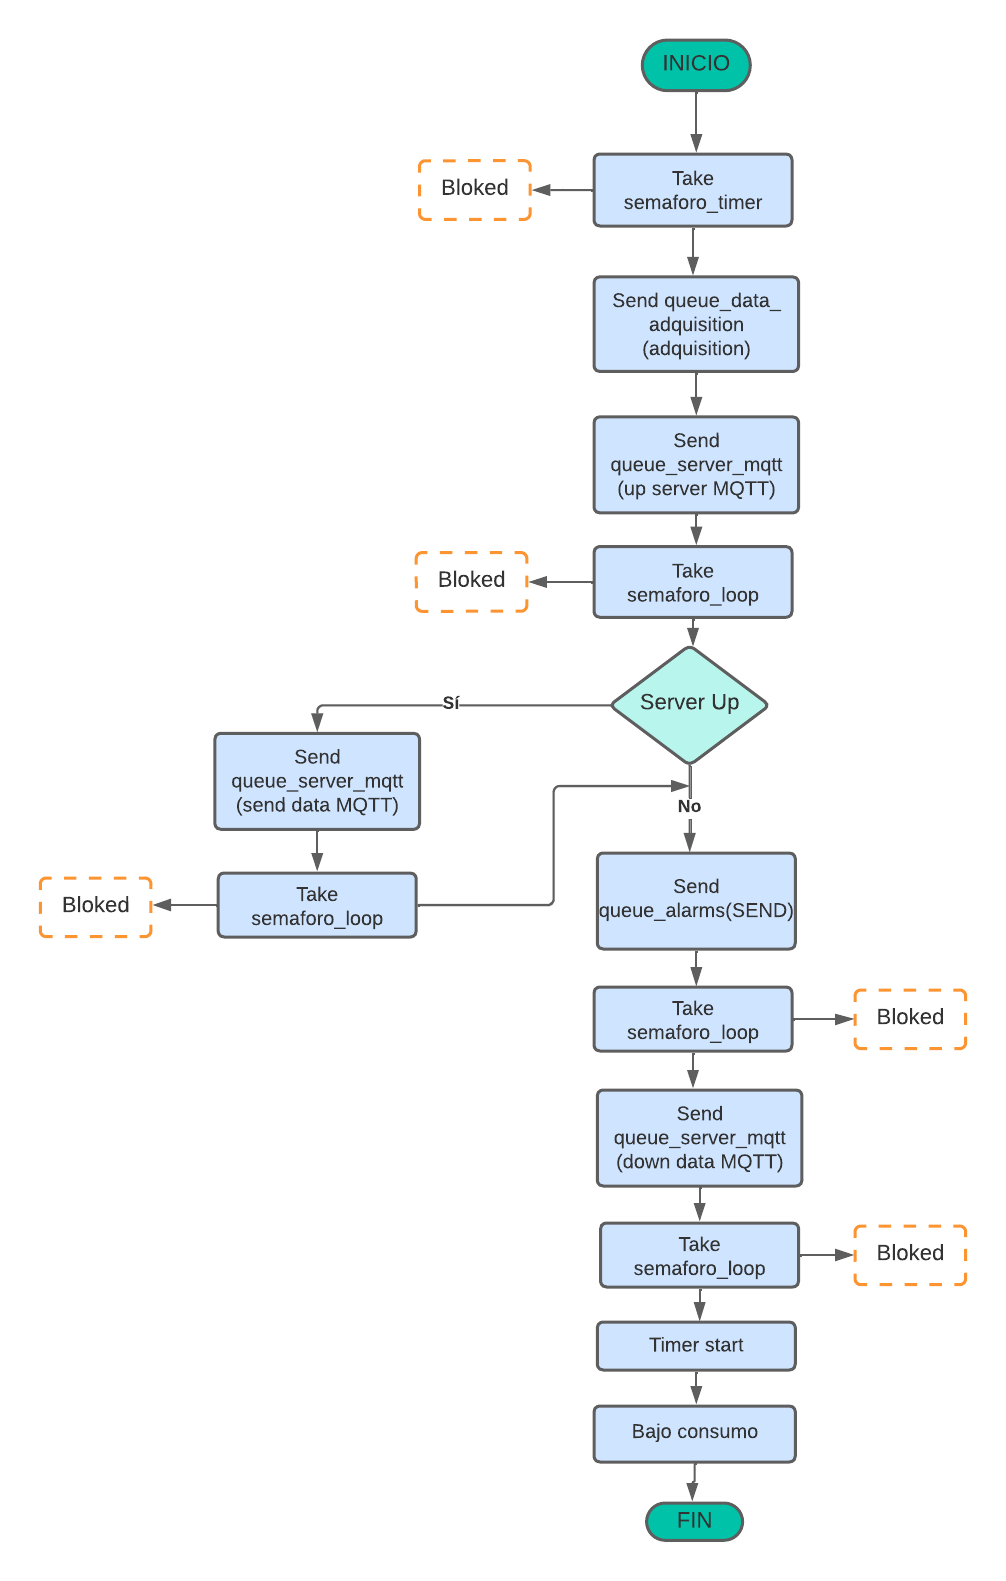
\includegraphics[width=12cm, height=14cm]{./Figures/DF task loop.png}
	\caption{Diagrama de flujo tarea loop.}
	\label{fig:Df tarea loop sistema}
\end{figure}

\clearpage
La figura \ref{fig:Df tarea adquisicion} muestra la secuencia repetiva que realiza la tarea de adquisicion de datos, la tarea inicia creando algunas variables locales que se utilizara en la tarea, luego entra al bucle infinito donde lo que promero que hace es ver si hay algun dato en la cola de adquisicion de datos si no hay se bloquea la tarea pero si hay realiza la lectura de todos los sensores, con los datos recolectados los envia a las colas de data y alarmas y termina el ciclo.
\begin{figure}[htbp]
  \centering
	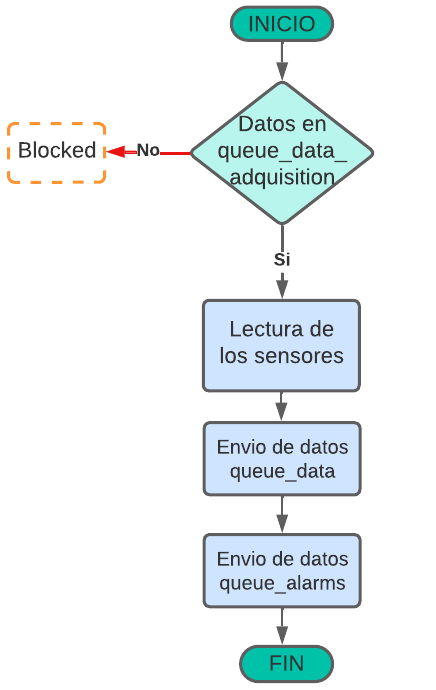
\includegraphics[width=6cm, height=7cm]{./Figures/DF task adquisicion.png}
	\caption{Diagrama de flujo tarea de adquisicion de datos.}
	\label{fig:Df tarea adquisicion}
\end{figure}

El manejo de las alarmas se realiza atraves de la tarea de alarmas la figura \ref{fig:Df tarea alarmas} describe la secuencia de la tarea, 
al entrar al bucle infinito lo primero que se realiza es revisar si existe algun dato en la cola de alarmas si no hay datos la tarea se bloquea hasta que alguien envie un dato a la cola, si hay dato se pregunta que evento contiene el dato resivido por la cola si es de monitorear lo que se hace es ver si el dato del sensor de humedad es menor al rango esperado si es asi se una variable en alto advirtiendo al sistema que hay una alarma, si se recicivio el evento de enviar se revisa si hay alarmas activas si hay se envia un mensaje de texto al 

\begin{figure}[htbp]
  \centering
	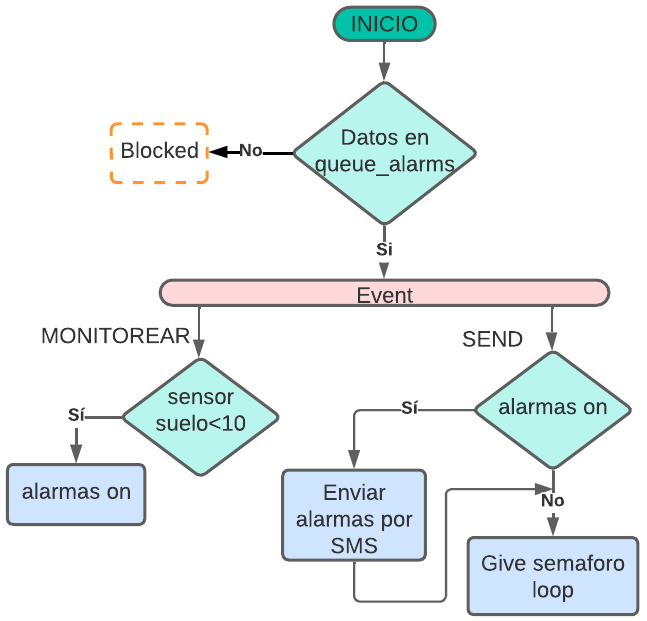
\includegraphics[width=6cm, height=6cm]{./Figures/DF_alarms.png}
	\caption{Diagrama de flujo tarea alarmas.}
	\label{fig:Df tarea alarmas}
\end{figure}

La ultima tarea que implento es la tarea que maneja la conexion del servidor que se describe en la figura 
La tarea comienza esperando datos en la cola de servidor mqtt si no hay datos la tarea se bloquea, si hay datos se revisa que evento es el que se recibio tenemos tres posibles eventos UP, DOWN y SEND ,
si recivimos el evento de UP la tarea entra a una maquina de estados pra levantar el servidor la figura muestra la maquina de estados del evento UP, si el evento es de DOWN la tarea ejecuta la maquina de estados que se ve en la figura y el evento es SEND la tarea espera que existan datos en la cola de data para haci armar la trama y publicar los datos al borker MQTT.

\begin{figure}[h]
  \centering
	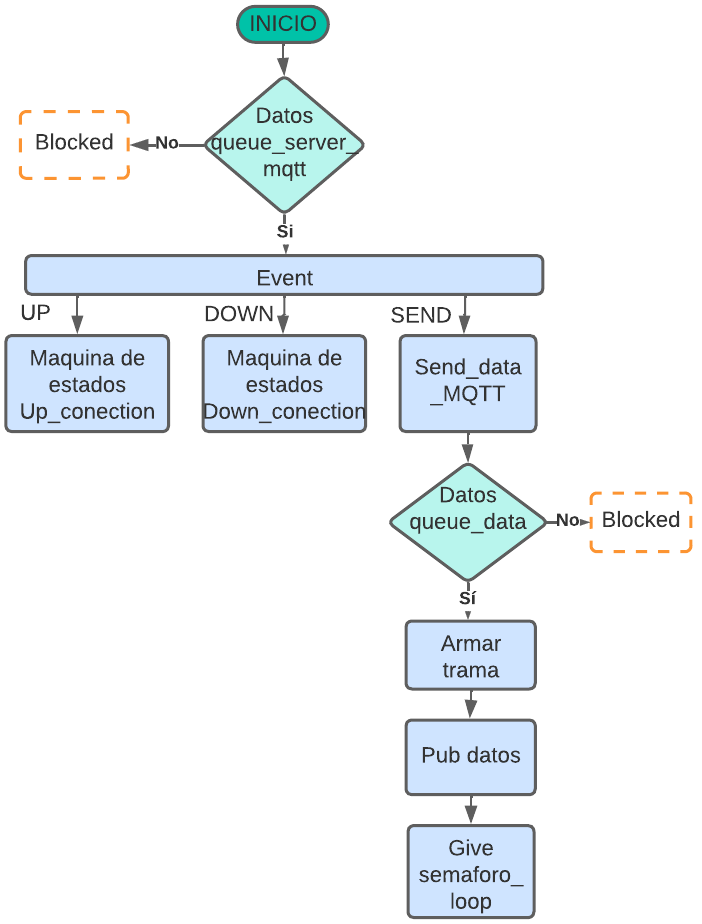
\includegraphics[width=8cm, height=8cm]{./Figures/DF general task conection.png}
	\caption{Diagrama de flujo tarea general conexion.}
	\label{fig:Df tarea conexion}
\end{figure}

\begin{figure}[h]
  \centering
  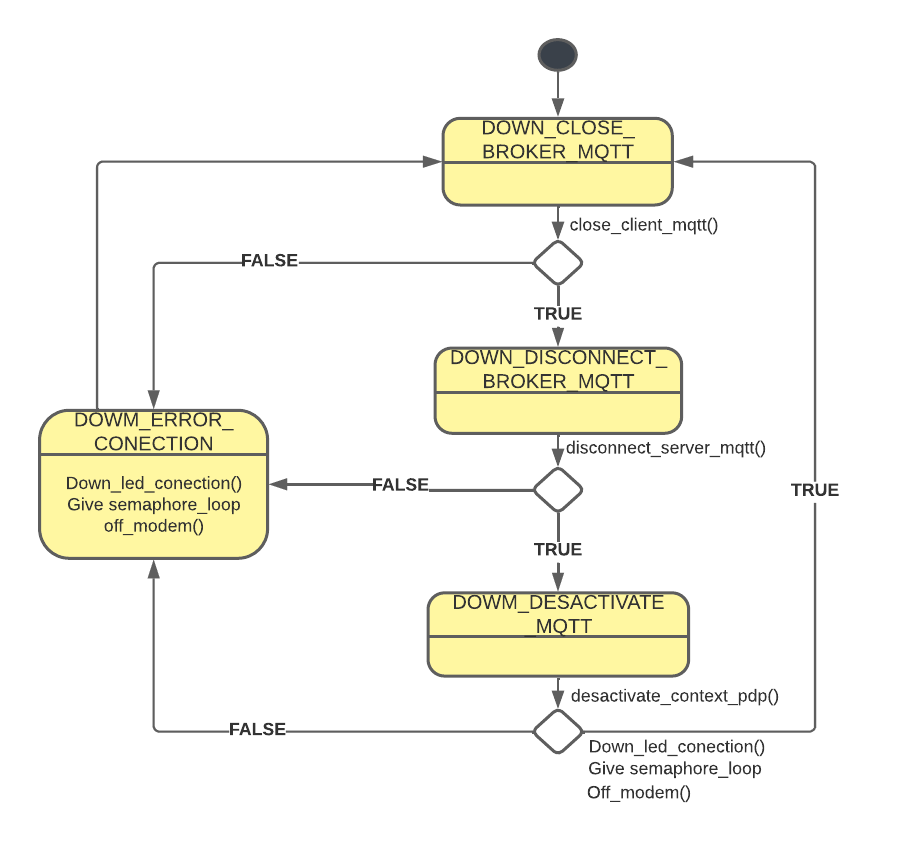
\includegraphics[width=8cm, height=8cm]{./Figures/SM down server.png}
  \caption{Maquina de estados dowm servidor.}
  \label{fig:Maquina de estados dowm servidor}
\end{figure}

\begin{figure}[h]
  \centering
	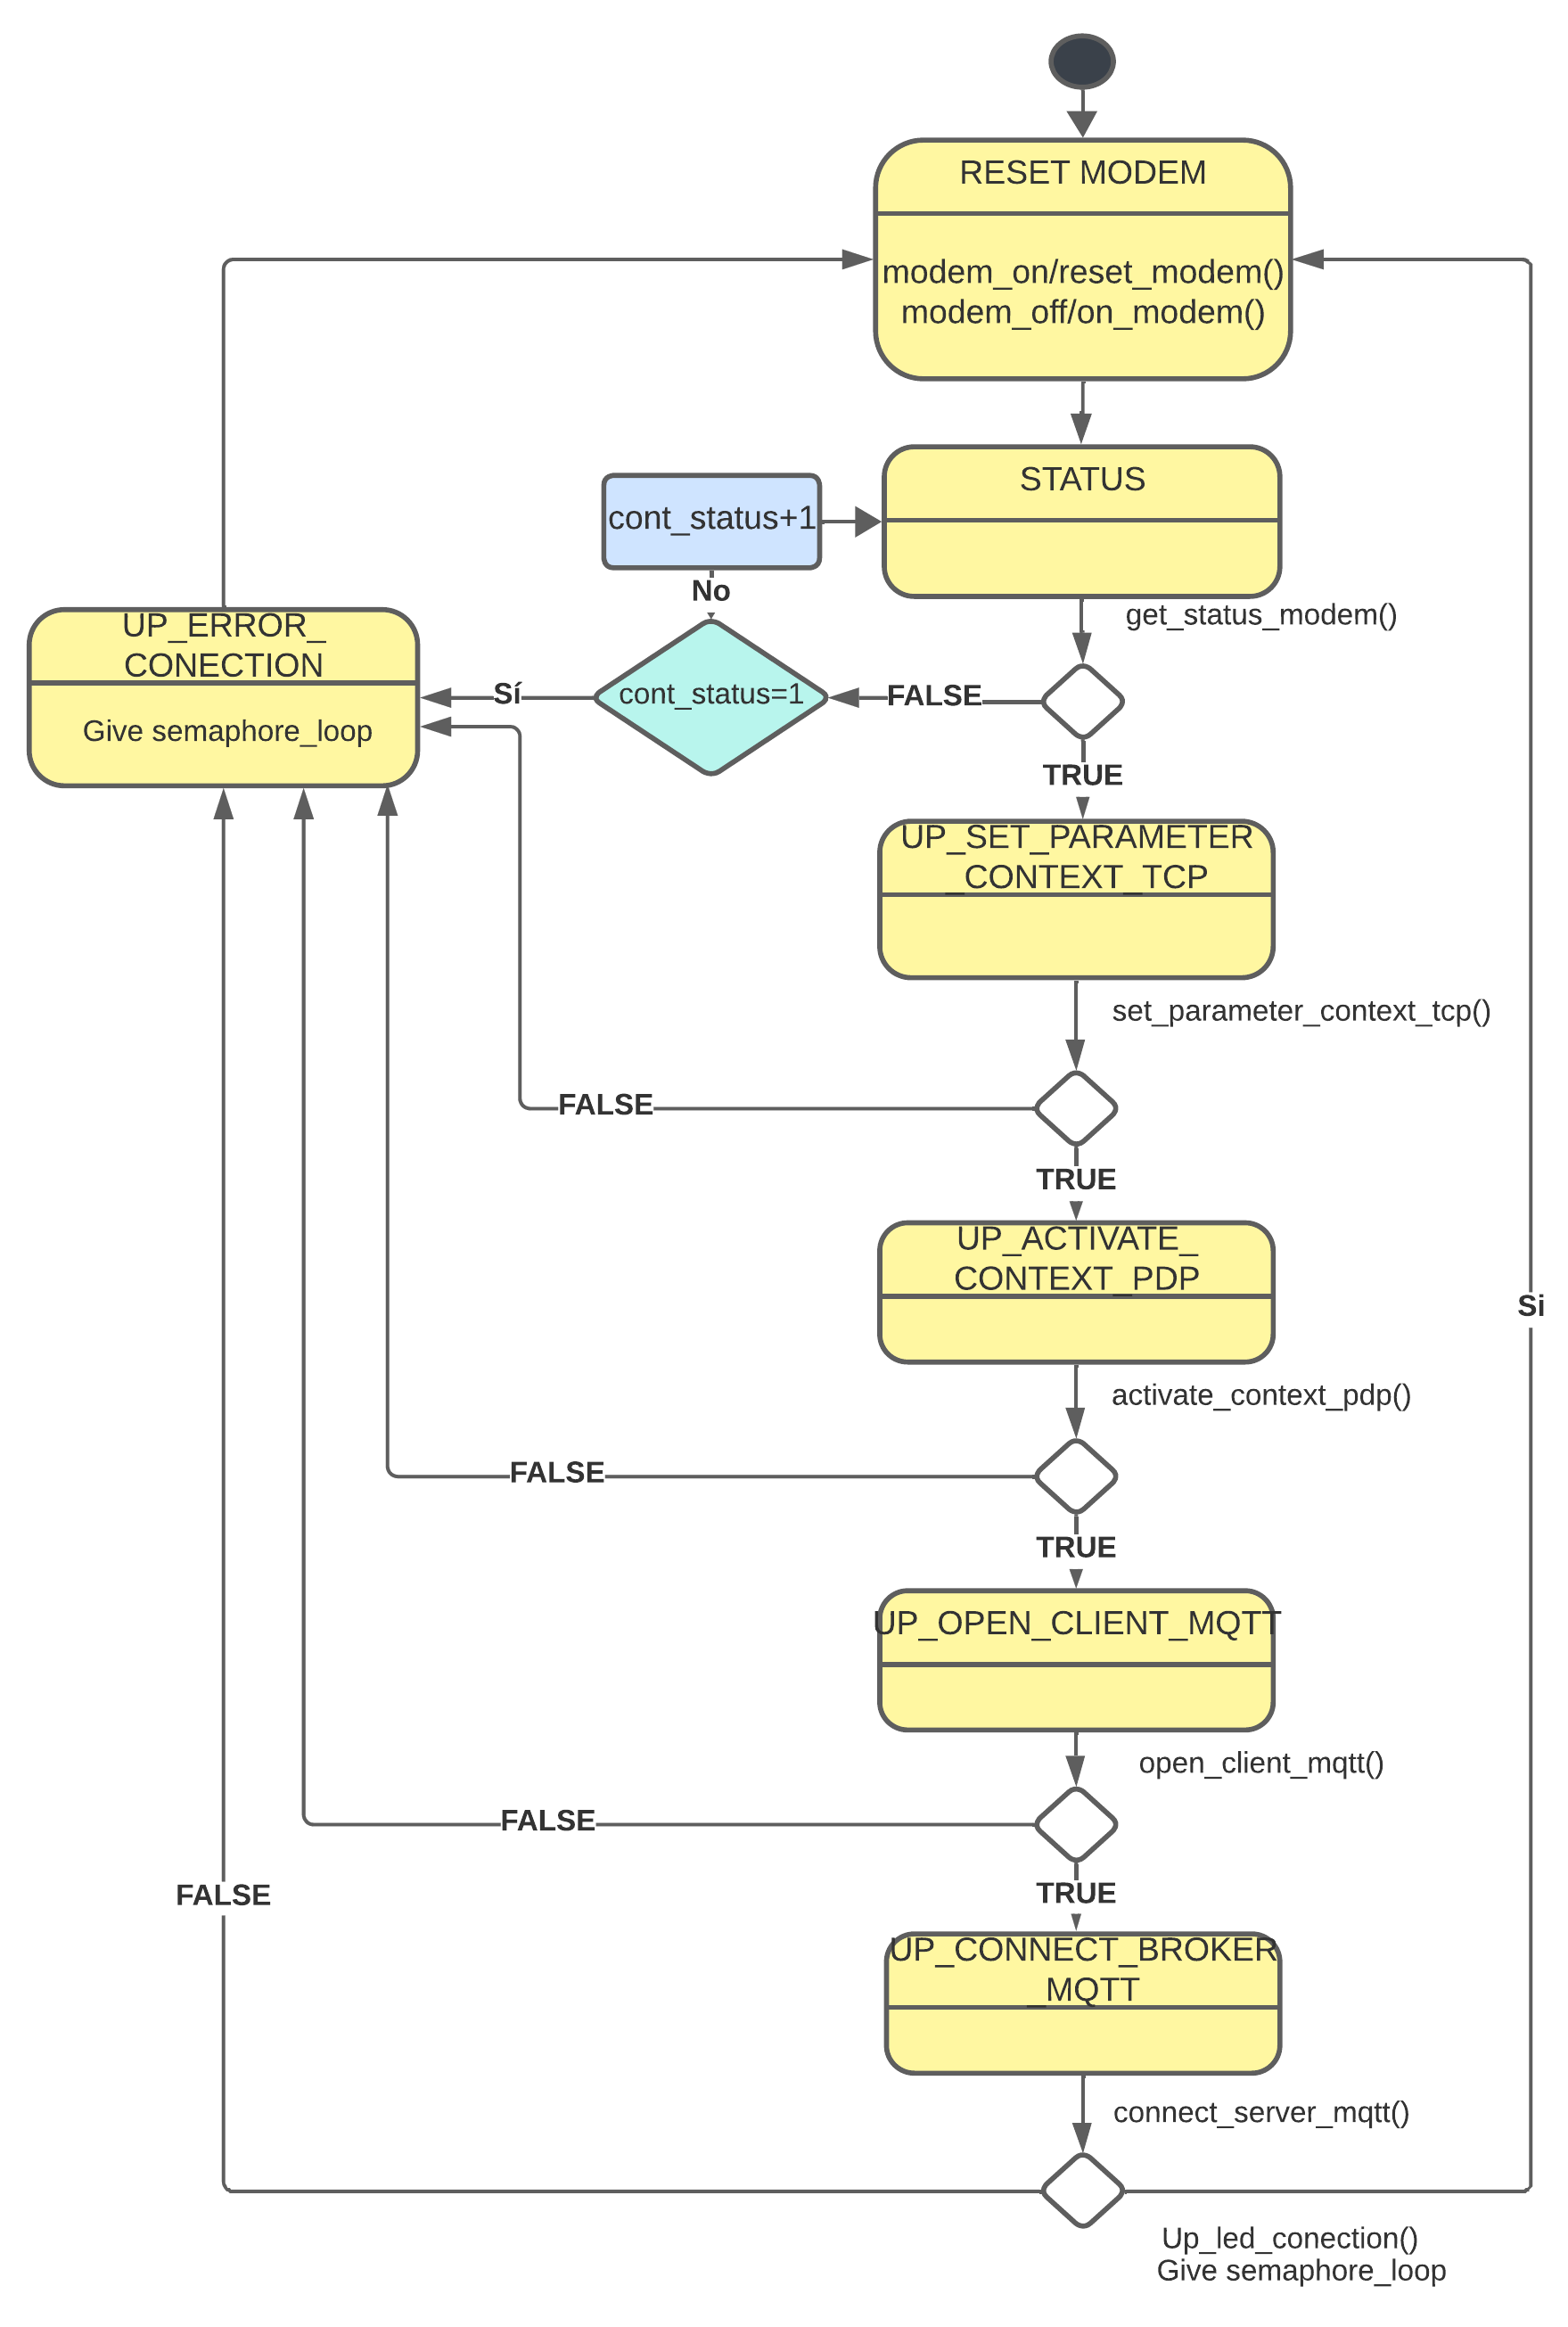
\includegraphics[width=10cm, height=15cm]{./Figures/SM up server.png}
	\caption{Maquina de estados up servidor.}
	\label{fig:Maquina de estados up servidor}
\end{figure}

\clearpage
\section{Controladores implementados}
Se implementaron dos controladores para el modulo de comunicacion BG96 y para el sensor de humedad y temperatura ambiente AHT-10
En el codigo se ven las funciones mas itilizadas del driver en el firmware.

\begin{lstlisting}[label=cod:vControl,caption=Funciones principales del driver del sensor AHT10.]  % Start your code-block

//!< Estructura para manejar los datos del driver del sensor    
typedef struct 
{
  aht10WriteFcn_t  writeI2C;
  aht10ReadFcn_t  readI2C;
  delay1ms_t      delay_ms_I2C;    
  aht10_status_fnc status_fun;
}aht10_config_t;

//!< Funcion para inicializar el driver 
void aht10Init(aht10_config_t *obj, aht10WriteFcn_t fncWritePort, aht10ReadFcn_t fncReadPort, delay1ms_t fncDelayPort)
{
  obj->writeI2C=fncWritePort;
  obj->readI2C=fncReadPort;
  obj->delay_ms_I2C=fncDelayPort;
}
//!< Funcion para lanzar una medicion
aht10_status_fnc aht10_launch_measurement(aht10_config_t *obj)
{
  uint8_t cmd[3] = {AHT10_CMD_TRIGGER_MEASUREMENT,AHT10_CMD_DATO_0,AHT10_CMD_DATO_1};
  obj->status_fun=AHT10_ERROR;
  obj->status_fun = obj->writeI2C(AHT10_ADDRESS_SLAVE ,cmd,3);
  if (obj->status_fun==AHT10_OK)
  {
    obj->delay_ms_I2C(AHT10_DELAY_LAUNCH_MEASUREMENT);
    if (aht10_get_status(obj)==SENSOR_IDLE)
    {
      obj->status_fun=obj->writeI2C(AHT10_ADDRESS_SLAVE,cmd,3);
      obj->delay_ms_I2C(AHT10_DELAY_LAUNCH_MEASUREMENT);
      return obj->status_fun;
    }
    else obj->status_fun=AHT10_ERROR;
  }
  return  obj->status_fun;
}
//!< Funcion para obtener el valor de la humedad del sensor 
aht10_status_fnc aht10_get_humedity(aht10_config_t*obj, uint8_t *data)
{
  
  if (obj== NULL)
  {
    return AHT10_ERROR;
  }
  obj->status_fun=AHT10_ERROR;
  uint8_t bufferRead[6]={0};
  uint32_t data_humedity=0;
  obj->status_fun=aht10_launch_measurement(obj);
  if (obj->status_fun==AHT10_OK)
  {
    obj->status_fun= obj->readI2C(AHT10_ADDRESS_SLAVE,bufferRead,6);
    if (obj->status_fun==AHT10_OK)
    {
      data_humedity=(((uint32_t)bufferRead[1]<<16) | ((uint16_t)bufferRead[2]<<8) | (bufferRead[3]))>>4;
      *data= HUMEDITY(data_humedity);
    }
  }
  return obj->status_fun;
}
//Funcion para obtener la temperatura obtenida por el sensor 
aht10_status_fnc aht10_get_temperature(aht10_config_t*obj, int8_t *data)
{
  if (obj== NULL)
  {
    return AHT10_ERROR;
  } 
  uint8_t buffer_read[6]={0};
  uint32_t data_temperature=0;
  obj->status_fun=AHT10_ERROR;
  obj->status_fun=aht10_launch_measurement(obj);
  if (obj->status_fun==AHT10_OK)
  {
    obj->status_fun=obj->readI2C(AHT10_ADDRESS_SLAVE ,buffer_read,6);
    if (obj->status_fun==AHT10_OK)
    {
      data_temperature=((uint32_t)(buffer_read[3] & 0x0F)<<16) | ((uint16_t) buffer_read[4]<<8)| buffer_read[5];
      *data= TEMPERATURE(data_temperature);
    }
  }
  return obj->status_fun;
}
\end{lstlisting}


Se implemento el driver del modulo de comunicacion.En el codigo se muestran las funciones mas utilizadas por el firmware del driver que son las de configuracion y activacion del APN, conexion y desconexion al servidor MQTT.


\begin{lstlisting}[label=cod:vControl,caption=Funciones principales del driver del sensor AHT10.]  % Start your code-block

typedef struct 
{
  em_status_modem  status_modem;
  em_state_server_mqtt_conection status_mqtt_server;
  pf_send_data    send_data_device;
  pf_reset_modem  f_reset_modem; 
  st_config_parameters_mqtt self_mqtt;
  st_config_context_tcp self_tcp;
  st_info_product info_product;
  uint8_t           last_error;
  char buffer_resp [100];
  char *current_cmd;
  em_bg96_error_handling ft_resp;
}st_bg96_config;
  
em_bg96_error_handling init_driver(st_bg96_config *self,pf_send_data ft_send_data_device,pf_reset_modem ft_reset_modem)
{
  if (ft_send_data_device!=NULL) {
    self->send_data_device=ft_send_data_device;
}
  if (ft_reset_modem!=NULL) {
    self->f_reset_modem=ft_reset_modem;
}
    self->status_modem=OFF;
    self->ft_resp=FT_BG96_OK;
    self->last_error=BG96_NO_ERROR;
    self->self_tcp.context_id=1;
    self->self_tcp.context_type=1;
    self->self_tcp.method_authentication=1;
    self->self_tcp.tcp_password="";
    self->self_tcp.tcp_username="";
    self->self_mqtt.identifier_socket_mqtt=0;
    self->self_mqtt.quality_service=0;
    self->self_mqtt.port=1883;
    self->self_mqtt.mqtt_client_id="123a56cb9";
    self->status_mqtt_server=SERVER_MQTT_DOWN;
    #ifdef UBIDOTS
    self->self_mqtt.host_name="\"industrial.api.ubidots.com\"";
    self->self_mqtt.mqtt_username="";
    self->self_mqtt.mqtt_password="";
    #endif
    #ifdef THINGS_BOARD
    self->self_mqtt.host_name="\"mqtt.thingsboard.cloud\"";
    self->self_mqtt.mqtt_username="";
    self->self_mqtt.mqtt_password="";
    #endif
    #ifdef MOSQUITTO
    self->self_mqtt.host_name="\"test.mosquitto.org\"";
    self->self_mqtt.mqtt_username="";
    self->self_mqtt.mqtt_password="";
    #endif
    #ifdef ENTEL
    self->self_tcp.tcp_apn="4g.entel";
    #endif
    #ifdef TIGO
    self->self_tcp.tcp_apn="internet.tigo.bol";
    #endif
  
    return self->ft_resp;
  }
  em_bg96_error_handling get_status_modem(st_bg96_config* self)
  {
      self->ft_resp=FT_BG96_OK;
      self->current_cmd="AT\r";
      self->ft_resp=self->send_data_device(self->current_cmd,RS_BG96_OK,self->buffer_resp,1000);
      if (self->ft_resp!=FT_BG96_OK)
      {
          self->last_error=BG96_ERROR_STATUS_MODEM;
      }
      return self->ft_resp;
  }
  
  
  
  em_bg96_error_handling send_sms_bg96(st_bg96_config *self,char*number,char*message)
  {
      self->ft_resp=FT_BG96_OK;
      char buffer_message[256];
      char buffer_number[20];
      sprintf(buffer_number,"AT+CMGS=\"%s\"\r",number);
      sprintf(buffer_message,"%s\x1a\r",message);
  
      self->ft_resp=self->send_data_device(buffer_number,RS_BG96_SIGNAL,self->buffer_resp,12000);
      if (FT_BG96_OK==self->ft_resp)
      {
          self->ft_resp=self->send_data_device(buffer_message,RS_BG96_OK,self->buffer_resp,12000);
          if (FT_BG96_OK!=self->ft_resp)
          {
              self->last_error=BG96_ERROR_SEND_SMS;
          }
      }
      return self->ft_resp;
  }
  
  em_bg96_error_handling set_parameter_context_tcp(st_bg96_config *self)
  {   
      self->ft_resp=FT_BG96_OK;
      char cmd[100];
      sprintf(cmd,"AT+QICSGP=%u,%u,\"%s\",\"%s\",\"%s\",%u\r",self->self_tcp.context_id,self->self_tcp.context_type,self->self_tcp.tcp_apn,self->self_tcp.tcp_username,self->self_tcp.tcp_password,self->self_tcp.method_authentication);
      self->ft_resp=self->send_data_device(cmd,RS_BG96_OK,self->buffer_resp,3000);
      if (self->ft_resp!=FT_BG96_OK)
      {
          self->last_error=BG96_ERROR_SET_PARAMETER_CONTEXT_TCP;
      }
      return self->ft_resp;
  }
  
  em_bg96_error_handling activate_context_pdp(st_bg96_config *self)
  {
      self->ft_resp=FT_BG96_OK;
      char cmd[30];
      sprintf(cmd,"AT+QIACT=%u\r",self->self_tcp.context_id);
      self->ft_resp=self->send_data_device(cmd,RS_BG96_OK,self->buffer_resp,15000);
      if (self->ft_resp!=FT_BG96_OK)
      {
          self->last_error=BG96_ERROR_ACTIVATE_CONTEXT_PDP;
      }
      return self->ft_resp;
  }
  
  em_bg96_error_handling desactivate_context_pdp(st_bg96_config *self)
  {
      self->ft_resp=FT_BG96_OK;
      char cmd[15];
      sprintf(cmd,"AT+QIDEACT=%u\r",self->self_tcp.context_id);
      self->ft_resp=self->send_data_device(cmd,RS_BG96_OK,self->buffer_resp,4000);
      if (self->ft_resp!=FT_BG96_OK)
      {
          self->last_error=BG96_ERROR_DESACTIVATE_CONTEXT_PDP;
      }
      return self->ft_resp;
  }
  em_bg96_error_handling set_parameters_mqtt(st_bg96_config *self)
  {
      self->ft_resp=FT_BG96_ERROR;
      char cmd_pdpid[30];
      sprintf(cmd_pdpid,"AT+QMTCFG=\"pdpid\",%u,%u\r",self->self_mqtt.identifier_socket_mqtt,self->self_tcp.context_id);
      self->ft_resp=self->send_data_device(cmd_pdpid,RS_BG96_OK,self->buffer_resp,300);
      if (self->ft_resp!=FT_BG96_OK)
      {
          self->last_error=BG96_ERROR_SET_PARAMETER_MQTT;
      }
      return self->ft_resp;
  }
  
  em_bg96_error_handling open_client_mqtt(st_bg96_config *self)
  {
      self->ft_resp=FT_BG96_ERROR;
      char cmd[100];
      sprintf(cmd,"AT+QMTOPEN=%u,%s,%u\r",self->self_mqtt.identifier_socket_mqtt,self->self_mqtt.host_name,self->self_mqtt.port);
      self->ft_resp=self->send_data_device(cmd,RS_BG96_CERO,self->buffer_resp,75000);
      if (self->ft_resp!=FT_BG96_OK)
      {
          self->last_error=BG96_ERROR_OPEN_CLIENT_MQTT;
  
      }
  
      return self->ft_resp;
  }
  em_bg96_error_handling close_client_mqtt(st_bg96_config *self)
  {
      self->ft_resp=FT_BG96_ERROR;
      char cmd[50];
      sprintf(cmd,"AT+QMTCLOSE=%u\r",self->self_mqtt.identifier_socket_mqtt);
      self->ft_resp=self->send_data_device(cmd,RS_BG96_OK,self->buffer_resp,3000);
      if (self->ft_resp!=FT_BG96_OK)
      {
          self->last_error=BG96_ERROR_CLOSE_CLIENT_MQTT;
      }
      return self->ft_resp;
  }
  
  em_bg96_error_handling connect_server_mqtt(st_bg96_config *self)
  {
      self->ft_resp=FT_BG96_ERROR;
      char cmd[150]={0};
      sprintf(cmd,"AT+QMTCONN=%u,\"%s\",\"%s\",\"%s\"\r",self->self_mqtt.identifier_socket_mqtt,self->self_mqtt.mqtt_client_id,self->self_mqtt.mqtt_username,self->self_mqtt.mqtt_password);
      self->ft_resp=self->send_data_device(cmd,RS_BG96_CERO,self->buffer_resp,10000);
      if (self->ft_resp!=FT_BG96_OK)
      {
          self->last_error=BG96_ERROR_CONNECT_SERVER_MQTT;
      }
     return self->ft_resp;
  }
  
  em_bg96_error_handling disconnect_server_mqtt(st_bg96_config *self)
  {
      self->ft_resp=FT_BG96_ERROR;
      char cmd[50]={0};
      sprintf(cmd,"AT+QMTDISC=%u\r",self->self_mqtt.identifier_socket_mqtt);
      self->ft_resp=self->send_data_device(cmd,RS_BG96_OK,self->buffer_resp,5000);
      if (self->ft_resp!=FT_BG96_OK)
      {
          self->last_error=BG96_ERROR_DISCONNECT_SERVER_MQTT;
      }
      return self->ft_resp;
  }
  
  
  em_bg96_error_handling publish_message(st_bg96_config *self,char *topic,char *data)
  {
      self->ft_resp=FT_BG96_ERROR;
      char cmd[50]={0};
      char buffer_data[220]={0};
      sprintf(buffer_data,"%s\x1a\r",data);
      sprintf(cmd,"AT+QMTPUB=%u,0,0,0,\"%s\"\r",self->self_mqtt.identifier_socket_mqtt,topic);
      self->ft_resp=self->send_data_device(cmd,RS_BG96_SIGNAL,self->buffer_resp,3000);
      if (FT_BG96_OK==self->ft_resp)
      {
          self->ft_resp=self->send_data_device(buffer_data,RS_BG96_CERO,self->buffer_resp,15000);
          if (self->ft_resp!=FT_BG96_OK)
          {
              self->last_error=BG96_ERROR_PUBLISH_MESSAGE;
          }   
      }
      else self->last_error=BG96_ERROR_PUBLISH_MESSAGE;
      return self->ft_resp;
  }


\end{lstlisting}
\clearpage
\section{Desarrollo del hardware}

Para el desarrollo del diseño del hardware se decidio utilizar como herramienta de diseño KICAD 6.0 por que es la herramienta que se aprendio en la especializacion.

\subsection{Esquematico} 
Lo que se hizo fue desarrollar un tarjeta donde se puedan conectar todos los modulos que se utilizaron para el prototipo
Al ser un prototipo no se realizon el diseño de un tarjeta con los compenentes mismo sino que se utlizaron modulo de desarrollo, lo que se hizo fue desarrollar un tarjeta donde se puedan conectar nuestros modulos utilizados como se el modulo celular, tarjeta de desarrollo STM32L432KC, los modulos sensores.

En la figura \ref{fig:esquematico root} se muestra la pagina raiz del esquematico del proyecto donde se puede ver la division del esquematico en 4 hojas, en la parte izquierda superior se ve el titulo de cada hoja en la parte derecha se ve la conexion entre las diferentes hojas, y en la parte izquierda inferior se ve el 3d del la tarjeta. 

\begin{figure}[h]
  \centering
	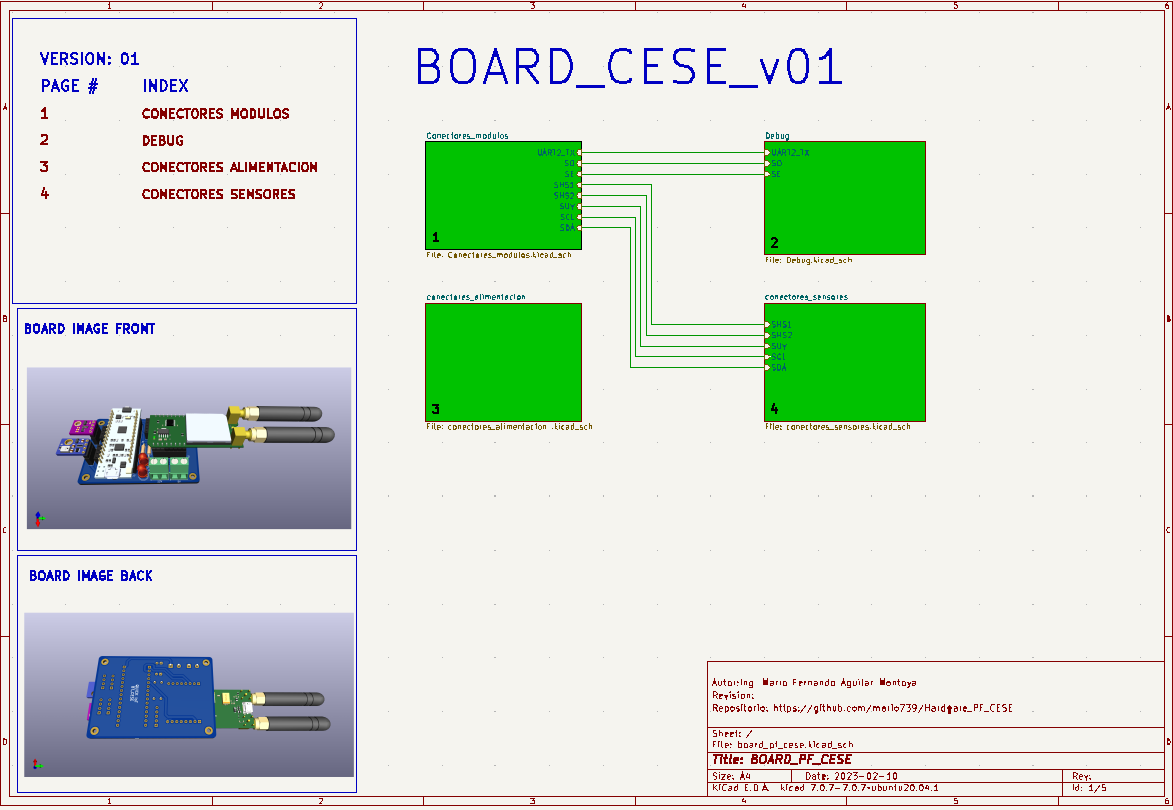
\includegraphics[width=\textwidth, height=10cm]{./Figures/esquematico_root.png}
	\caption{Esquematico pagina root.}
	\label{fig:esquematico root}
\end{figure}
\clearpage
Para el diseño del shield se consideraron las medidas de la modulos que se conectarian,en la figura \ref{fig:esquematico modulos} se muestra los dos conectores de los modulos mas importantes el modulo de comuicacion BG96, modulo NUCLEO-L432KC y las conexiones entre ellos.

\begin{figure}[h]
  \centering
	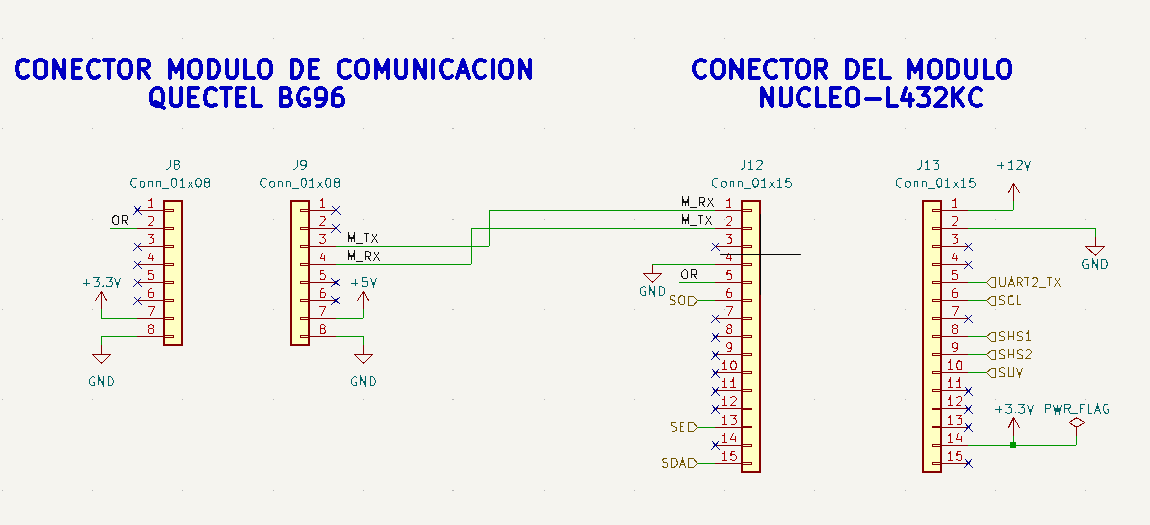
\includegraphics[width=\textwidth, height=8cm]{./Figures/esquematico_modulos.png}
	\caption{Esquematico conectores modulos.}
	\label{fig:esquematico modulos}
\end{figure}

Se colocaron dos leds para debug, uno para senalizar si se logro conectar al servidor MQTT y el otro led para senalizar si el sistema entra en un estado de error, se coloco un conector para una puerto serial por donde el modulo manda la secuencias de comandos que manda y recive al modulo de comunicacion.En la figura \ref{fig:esquematico conectores de debug} se puede ver el circuito.
\begin{figure}[h!]
  \centering
	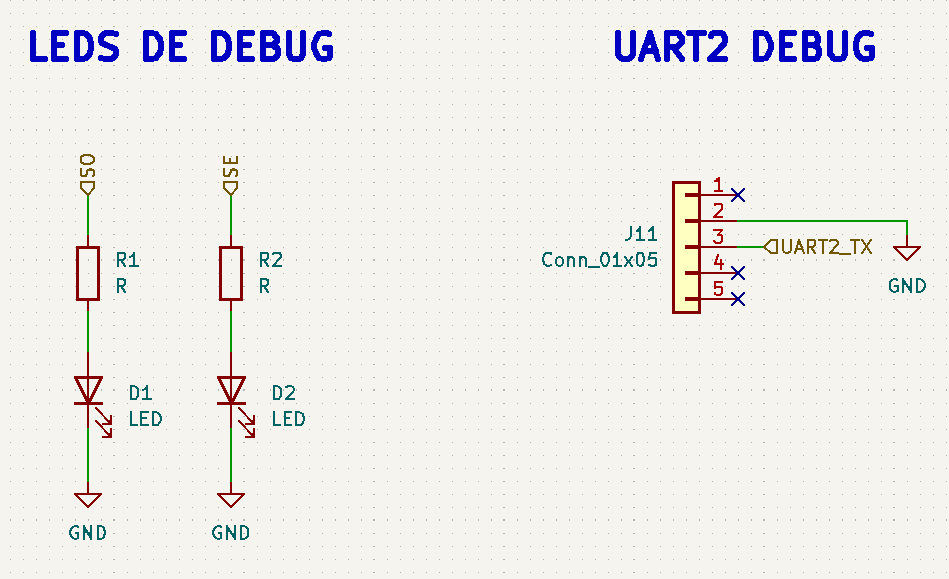
\includegraphics[width=\textwidth, height=7cm]{./Figures/esquematico_debug.png}
	\caption{Esquematico interfaz de debug.}
	\label{fig:esquematico conectores de debug}
\end{figure}
\clearpage
En la figura \ref{fig:esquematico conectores sensores} se pueden ver los conectores que se pusieron a la placa para conectar los sensores del nodo: sensor de humedad 1, sensor de humedad 2, sensor de luz UV y el sensor de humedad y temperatura ambiente AHT-10.

\begin{figure}[h]
  \centering
	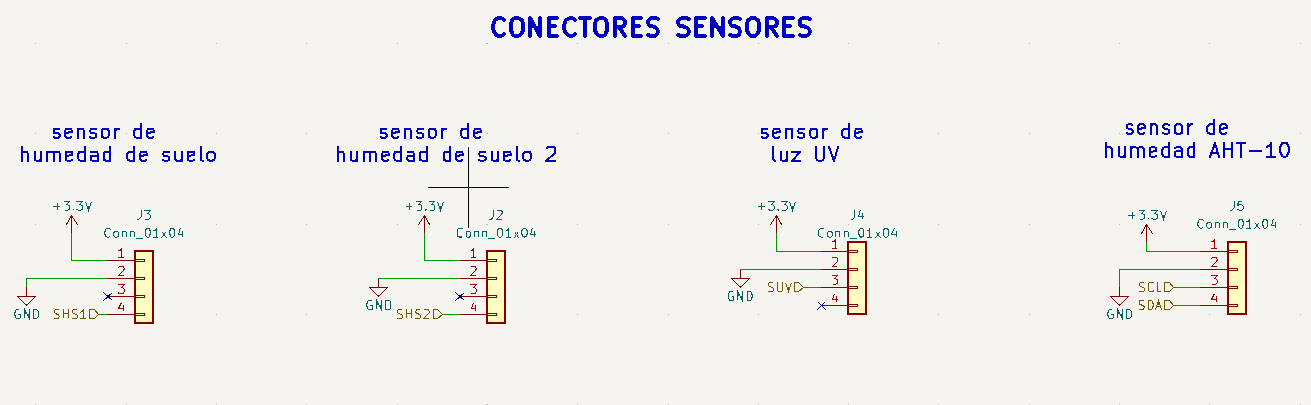
\includegraphics[width=\textwidth, height=8cm]{./Figures/esquematico_conectores_sensores.png}
	\caption{Esquematico conectores sensores.}
	\label{fig:esquematico conectores sensores}
\end{figure}

Se colocaron dos colectores de alimentacion como se muestra en la figura \ref{fig:esquematico conectores alimentacion}, el conector de 12 v para alimentar al modulo del microcontroaldor y el otro conector para alimentar al modulo de comunicacion.
\begin{figure}[h]
  \centering
	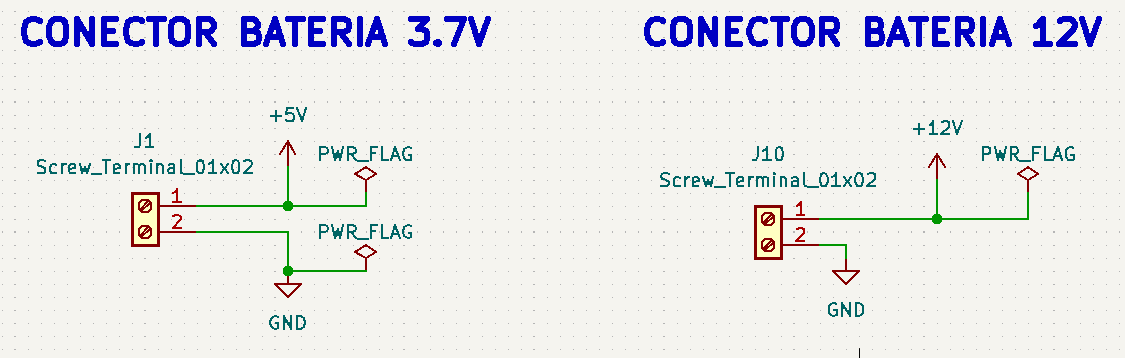
\includegraphics[width=\textwidth, height=8cm]{./Figures/esquematico_alimentacion.png}
	\caption{Esquematico conectores alimentacion.}
	\label{fig:esquematico conectores alimentacion}
\end{figure}
\clearpage
\subsection{PCB del hardware} 
La figura muestra el circuito impreso diseñado para el proyecto.

\begin{figure}[h!]
  \centering
  \begin{subfigure}[b]{0.45\linewidth}
  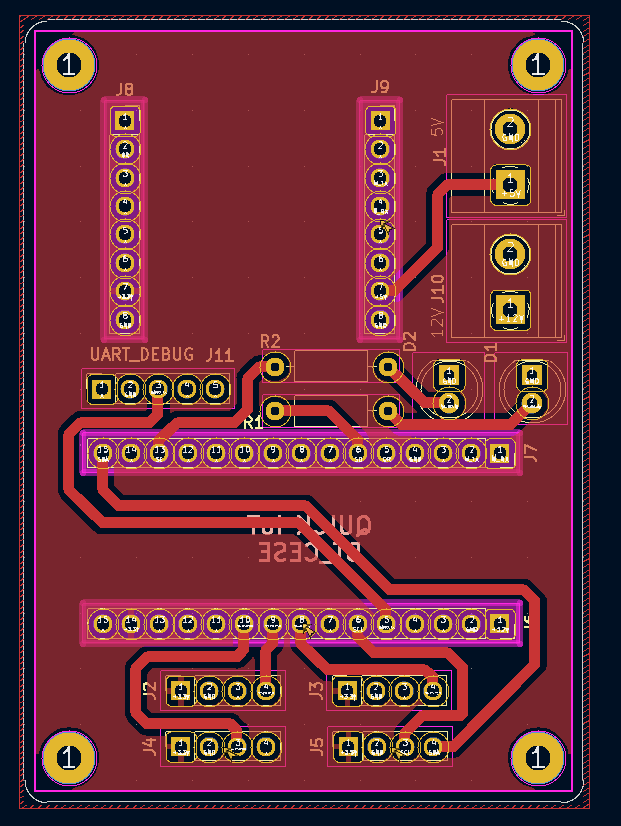
\includegraphics[width=\linewidth]{./Figures/pcb_top.png}
  \caption{Capa top PCB}
  \label{fig:Capa top PCB}
  \end{subfigure}
  \begin{subfigure}[b]{0.44\linewidth}
  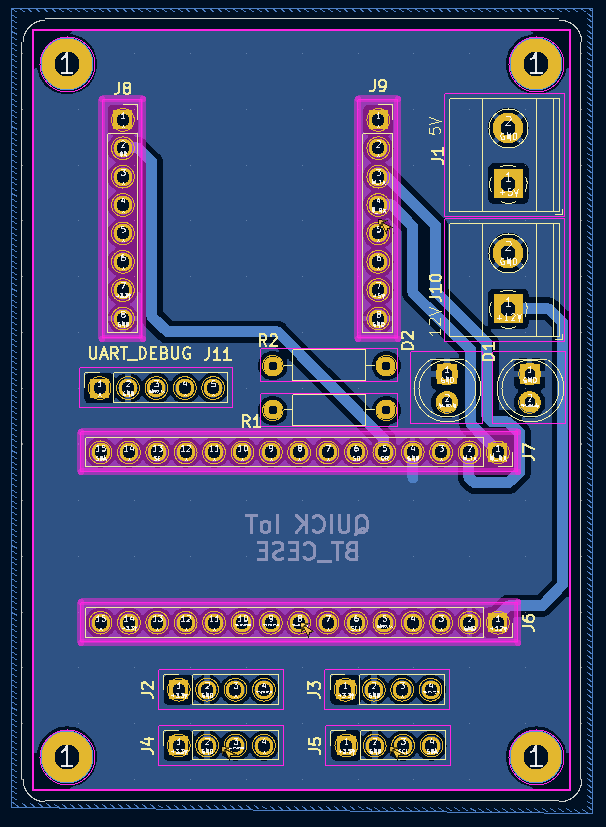
\includegraphics[width=\linewidth]{./Figures/pcb_bot.png}
  \caption{Capa bot PCB}
  \label{fig:Capa bot PCB}
  \end{subfigure}
  \caption{PCB del proyecto.}
  \label{fig:PCB del proyecto}
  \end{figure}

En la figura se muestra del diseno de la tarjeta del circuito impreso en 3D.
\begin{figure}[h!]
  \centering
	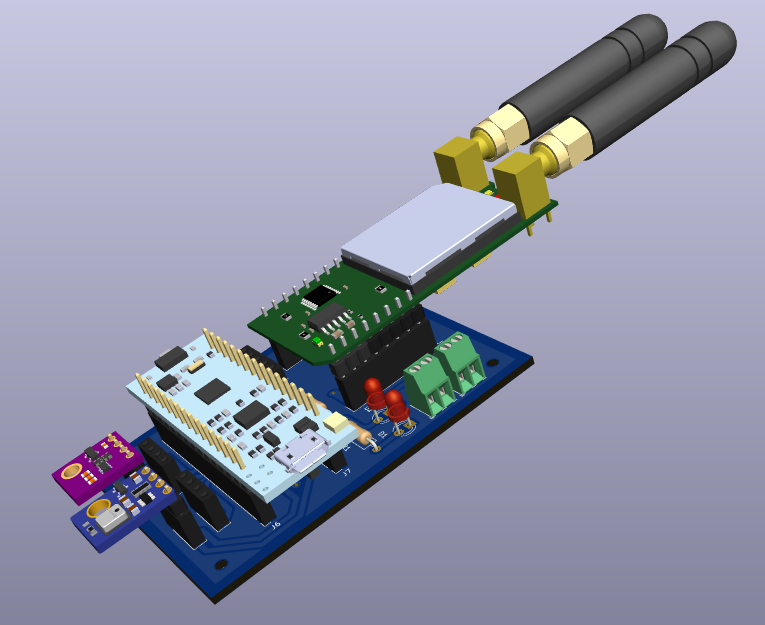
\includegraphics[width=\textwidth, height=8cm]{./Figures/tarjeta3d.png}
  \caption{3D del tarjeta desarrollada.}
	\label{fig:3D del modulo}
\end{figure}


\clearpage
\section{Paneles de visualizacion}
La herramienta de visualizacion de ThingsBoard es muy versatil para el armado de paneles de visualizacion escalables y altamente configurables.

Se armaron dos paneles de visualizacion un panel principal que muestra todos los nodos sensores implementados y un panel secundario o panel de nodo sensor que muestra de forma detallada las variables monitoreadas por el nodo sensor.
\subsection{Panel principal} 

En la figura \ref{fig:Panel principal} se aprecia el panel principal de la interfaz grafica.A continuación se describira cada zona del panel principal.
El panel esta dividido en las siguientes zonas:
\begin{itemize}
  \item Zona 1: Listado de todos los nodos sensores implementados y activos, asiendo click en el dispositivo podemos navegar al panel de visualizacion del nodo donde podemos ver con mas detalle las variables medidas.
  \item Zona 2: Graficas que muestra los cambios que van teniendo los valores de las variables medidas por los sensores con respecto al tiempo.
  \item Zona 3: Mapa con la ubicacion de los nodo sensores implmentados.
\end{itemize}

\begin{figure}[h]
  \centering
	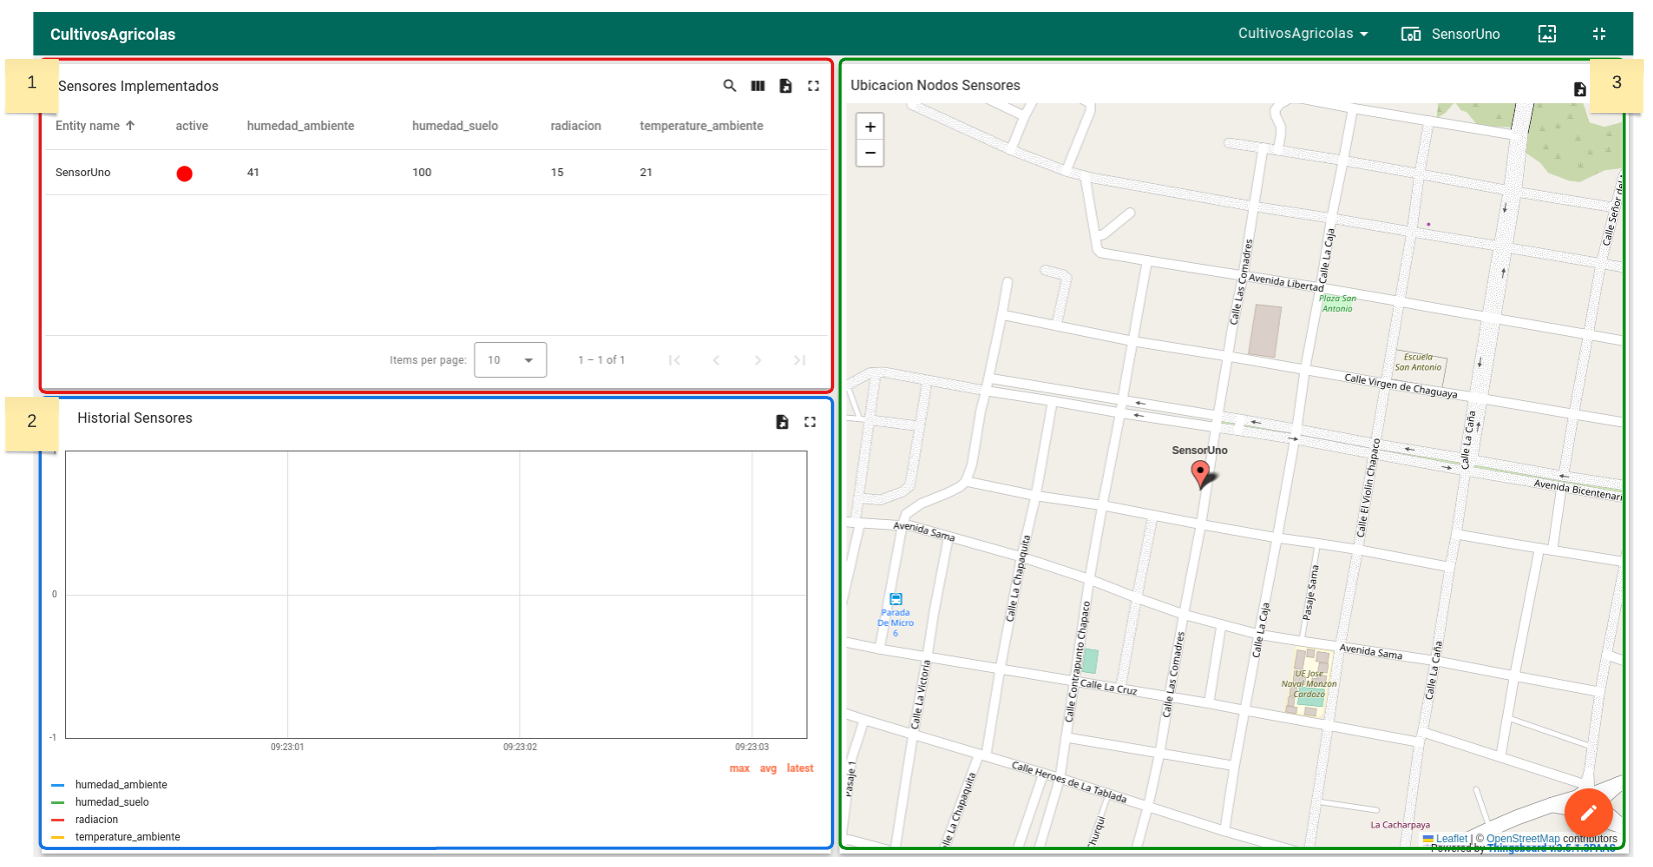
\includegraphics[width=\textwidth, height=11cm]{./Figures/panel_principal_editado.png}
  \caption{Panel principal de la interfaz grafica.}
	\label{fig:Panel principal}
\end{figure}

\clearpage
\subsection{Panel nodo sensor} 

Para tener un mayor detalle de todos los parametros de monitoreo de cada nodo sensor se creo un panel secundario que se muestra en la figura \ref{fig:Panel nodo sensor}.

El panel esta dividido en las siguientes zonas:
\begin{itemize}
  \item Zona 1: Graficas que muestra los cambios que van teniendo los valores de las variables medidas por los sensores con respecto al tiempo.
  \item Zona 2: Widgets que muestran el ultimo valor obtenido por el nodo sensor de cada variable monitoreada.
  \item Zona 3: Tabla que monitorea las alarmas implementadas. 
  \item Zona 4: Se tiene un mapa que muestra la ubicacion del nodo sensor.
\end{itemize}

\begin{figure}[h!]
  \centering
	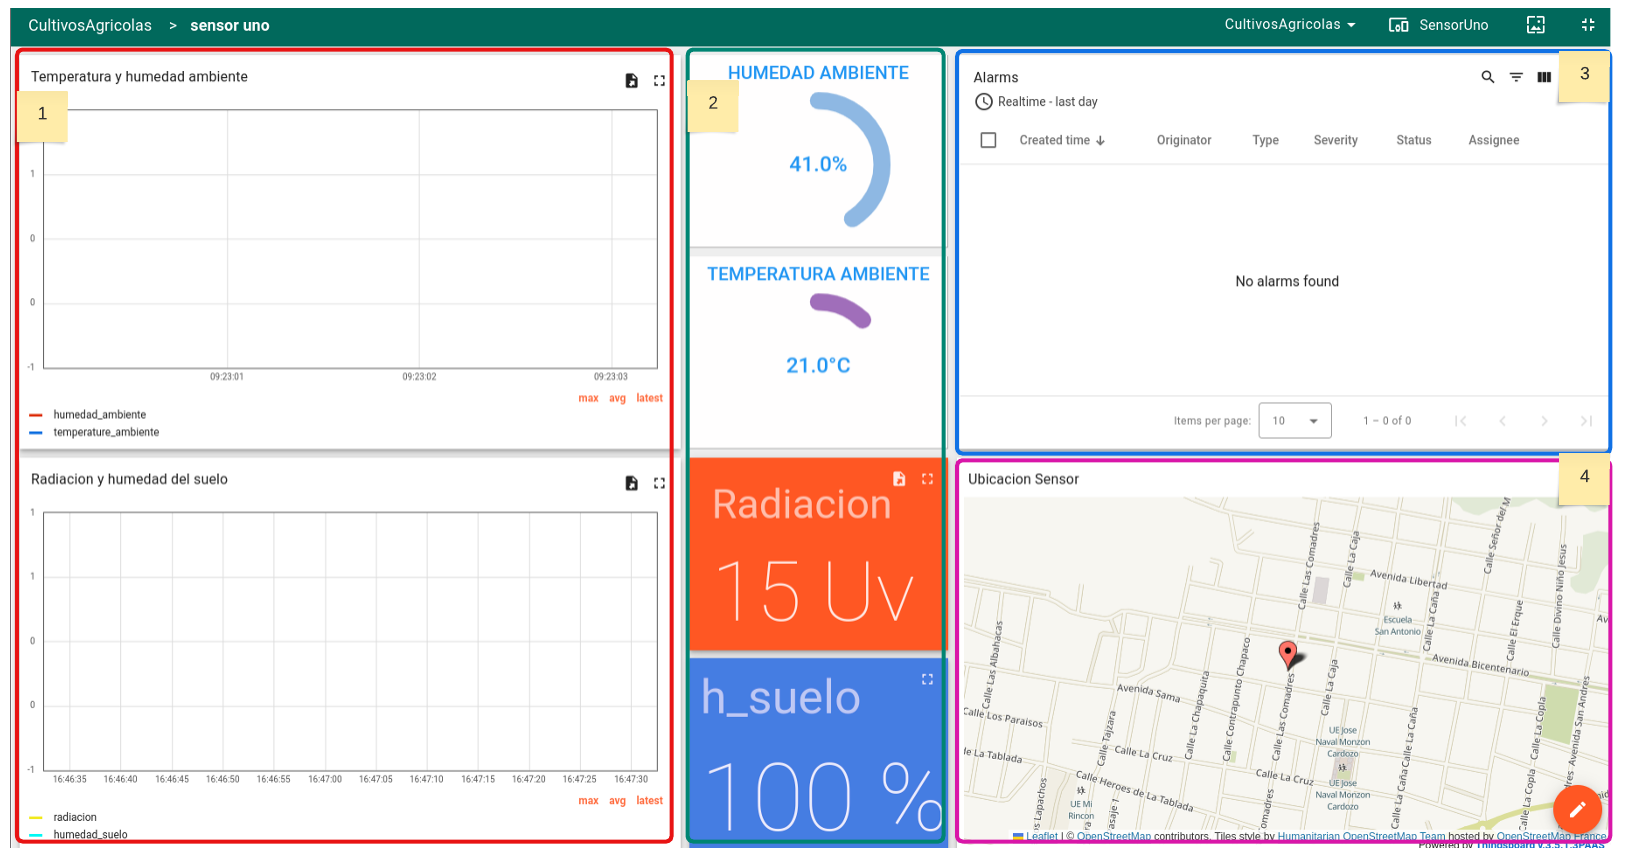
\includegraphics[width=\textwidth, height=8cm]{./Figures/panel_nodosensor_editado.png}
  \caption{Panel nodo sensor.}
	\label{fig:Panel nodo sensor}
\end{figure}